Прежде чем создавать свою предсказательную систему следуют хорошо изучить предметную область и разобраться, какого рода данные будут в неё поступать. Специалистам по машинному обучению части приходится подробно углубиться в новую для них область знаний, определить закономерности во входных данных, определить, как их подготовить и какими методами потом обрабатывать.

Входные данные могут быть представлены весьма разнообразными способами: набором фотографий, видео или аудиофайлов, в виде текста, например, сообщений пользователей, отзывов покупателей, переписки или писем, в виде электронных таблиц. Обычно исходное представление не удобно и не может быть непосредственно использовано для обработки, и если компьютер работает с числами, то человеку удобнее мыслить визуальными образами. Визуализация служит именно этим целям.

Визуализация (от лат. visualis, «зрительный», англ. Visualization)~— общее название приёмов представления числовой информации или физического явления в виде, удобном для зрительного наблюдения и анализа\cite{wiki:visualization_def}.

Пионером в области визуализации считается Шарль Жозеф Минар (27 марта 1781, Дижон~— 24 октября 1870, Бордо). На \autoref{minar-visio} представлены карты, сделанные им: от 29 ноября 1869 года — графическая визуализация вторжения Наполеона Бонапарта в Россию в 1812 году и от 20 ноября 1869 года~— карта, показывающая перемещение войск Ганнибала из Иберии (Испании) в Италию во время Второй Пунической войны.

\begin{figure}[H]
    \centering
    \includegraphics[width=\textwidth]{chapter1/minard_map_book.jpg}    
    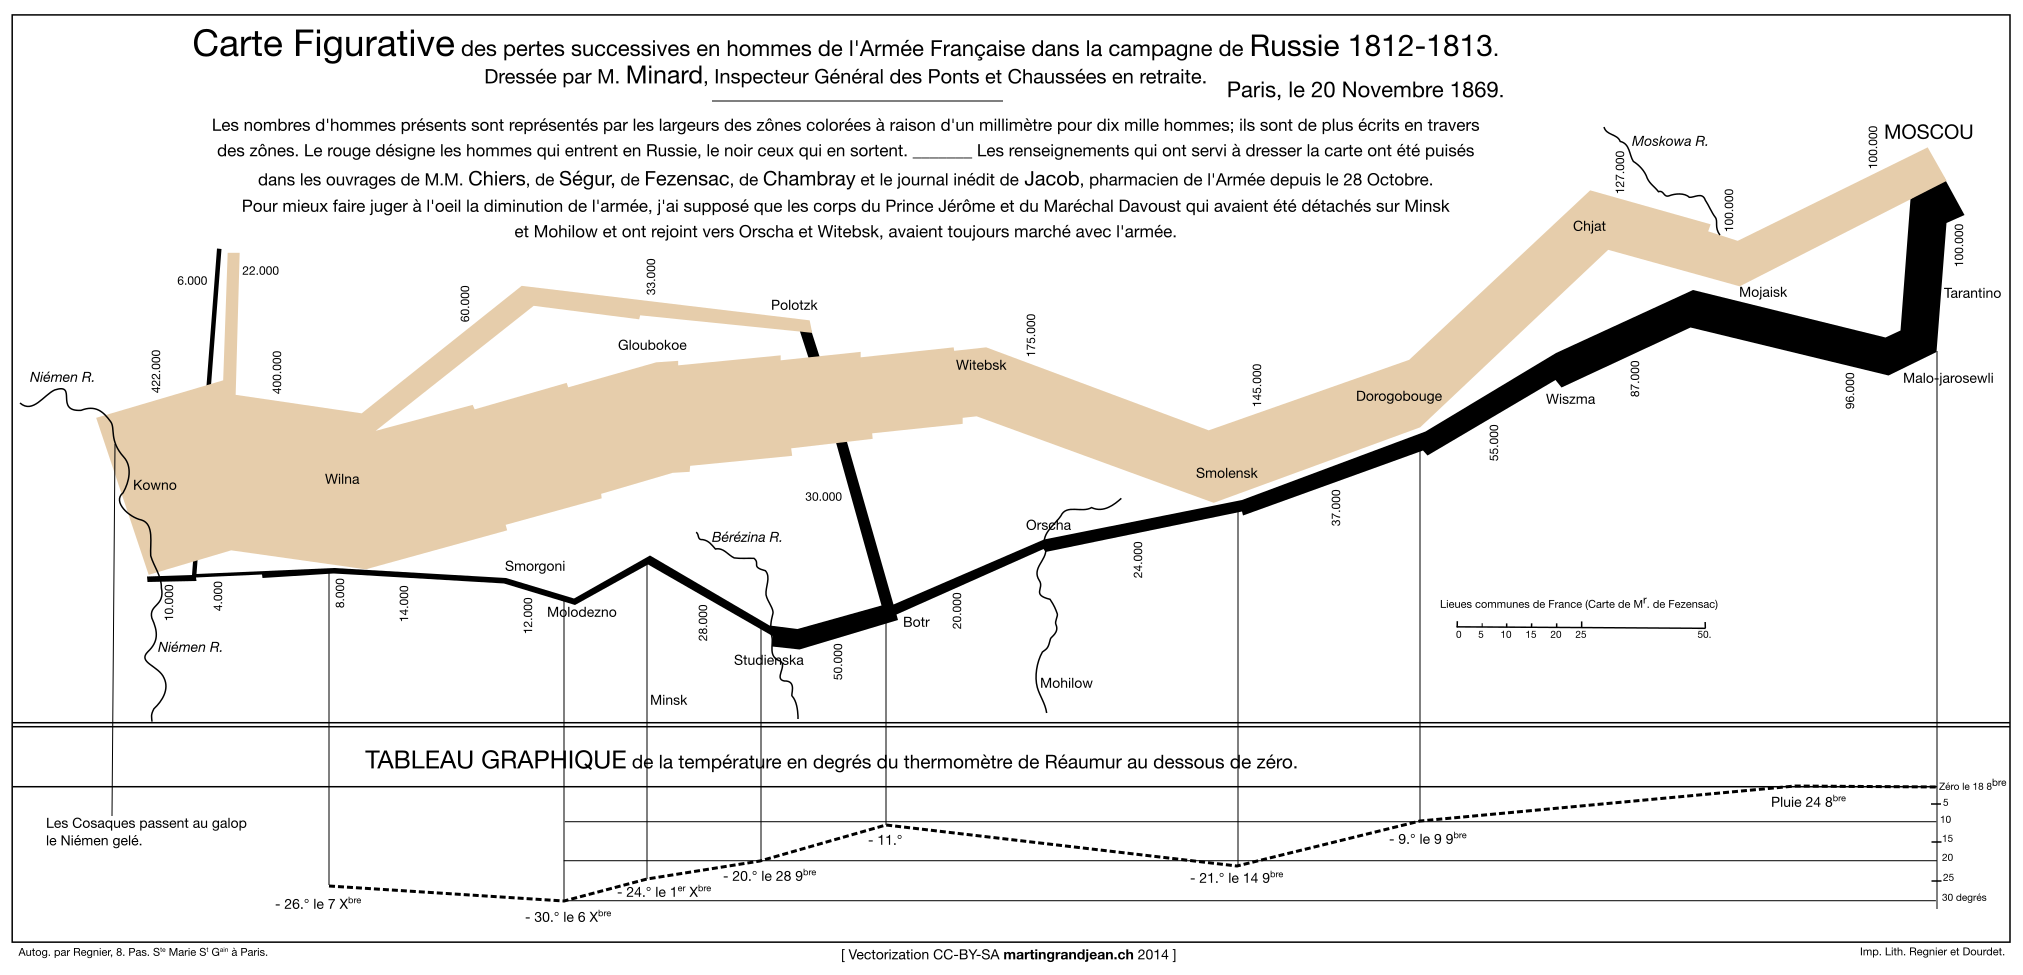
\includegraphics[width=\textwidth]{chapter1/Minard's_Map.png}
    \caption{Визуализации Минара. Оригинальная и современная версии}
    \label{minar-visio}
\end{figure}

Особенный интерес представляет карта вторжения Наполеона, на этой карте изображено огромное количество информации. Толщина линии соответствует размеру армии, цвет~\--- направлению (коричневый~\--- наступлению на Москву, а чёрный~\--- отступлению, на карте подписаны названия городов, через которые проходила армия, дата и температура воздуха по шкале Реомюра, а также расстояние между этими городами). Достаточно лишь одного взгляда на карту, чтобы увидеть, какие последствия этот поход имел для армии Наполеона, но не только это, а так же и пройденное расстояние, города, даты и погоду. И вся эта информация, которой достаточно для составления хорошего справочника, помещается на одной картинке, что значительно ускоряет и облегчает её усвоение.

При составлении карты была проделана огромная работа и по сбору информации и по составлению визуализации и её печати, и всё это без современных графических редакторов и средств типографии. Нам сейчас гораздо проще и собирать информацию и выводить её, но всё равно, визуализация требует значительных затрат времени и сил, но она того стоит, зачастую лучше потратить дополнительные силы на хорошую визуализацию, чем переходить к написанию кода, потому что понимание структуры данных и имеющихся в них закономерностях способно значительно облегчить написание программы, и увеличить её эффективность.

Допустим, перед вами поставили задачу определить насколько неудачен был поход Наполеона в Российскую империю и предположить, какие факторы послужили причиной. Идеи, которые первыми придут в голову, зачастую оказываются ошибочными, например, можно посмотреть потери обеих армий в ходе сражения, однако, это даст лишь совсем грубую оценку, потому что мы не учитываем потери на марше, от болезней, голода и холода, кстати, насчёт холода. Есть распространённое суждение, что Россию невозможно захватить зимой, и все неудачи завоевателей объясняются лишь климатом. 

Не вдаваясь в исторические аналогии с монголами, которые прошлись по Руси как раз таки зимой и не сравнивая наступления 1812 года и 1941 (армия наполеона вошла в Москву 2 (14 по старому стилю) сентября, в это же время в 1941 году происходило сражение за Смоленск, а начинали они почти одновременно), а лишь глядя на визуализацию Минара можно заметить, что основные потери армия понесла в ходе наступления на Москву, которое осуществлялось летом, до Москвы дошли лишь 100 тыс из 422 тыс, перешедших границу (среди историков до сих пор не утихают споры о точном размере вторгшийся армии и её потерях, но, что она уменьшилась в разы сходятся все), а сравнив размеры вторгшийся армии и отступившей её части, понятно, насколько значительны были потери.

Это историческое отступление было сделано для того, чтобы вам была понятны все возможности, которые открывает хорошая визуализация, а именно, возможность быстро сделать правильные выводы, надеюсь, это послужило достаточным обоснование и мотивацией для вас в создании визуализаций.

Очень часто данные представлены в табличном виде, обычно каждая строка~\-- это объект, а столбец~\-- какой-то признак\autoref{tables-representation}. Если же вы ещё недостаточно убеждены в полезности визуализаций, возможно, взгляд на этот рисунок склонит вас на светлую сторону силы.

\begin{figure}[H]
    \centering    
    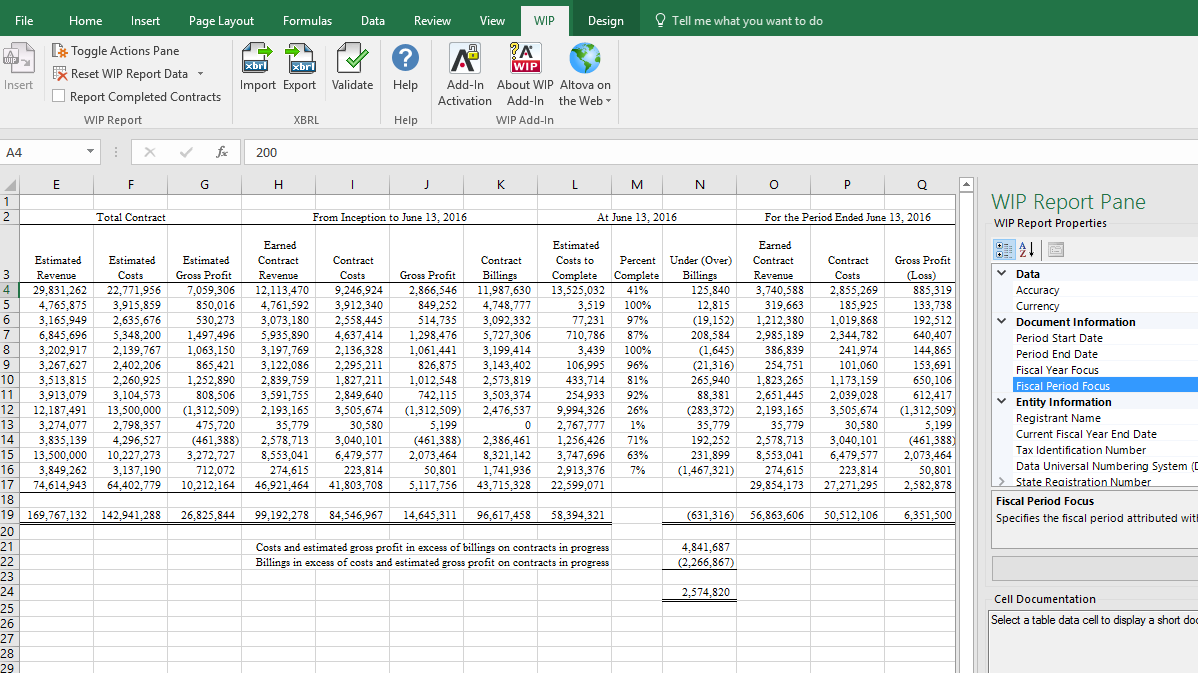
\includegraphics[width=\textwidth]{chapter1/tables-in-excel.png}    
    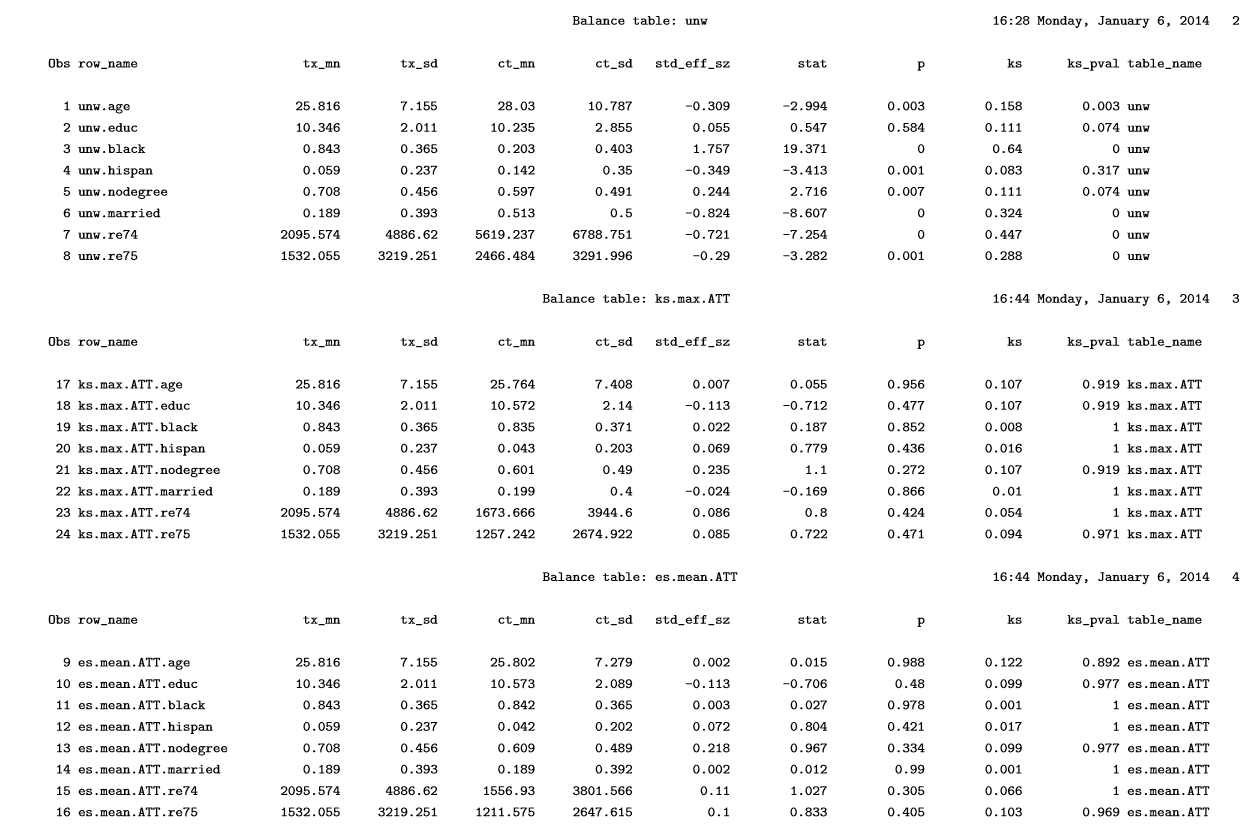
\includegraphics[width=\textwidth]{chapter1/huge-table.jpg} % SAS Macros Tutorial - https://www.rand.org/statistics/twang/sas-tutorial.html
    \caption{Представление данных в виде таблиц}
    \label{tables-representation}
\end{figure}

Настало время попробовать самим. 

\begin{wrapfigure}{r}{0.33\textwidth}
    \vspace{-0.5cm}
    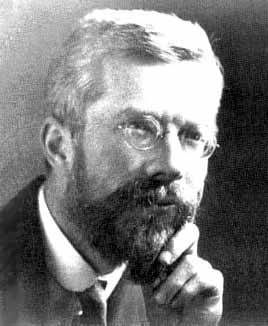
\includegraphics[width=\linewidth]{chapter1/Fischer.jpg}
     %https://upload.wikimedia.org/wikipedia/commons/4/46/R._A._Fischer.jpg
\end{wrapfigure}
Рональд Фишер в 1936 году продемонстрировал работу разработанного им метода анализа. Данные были собраны американским ботаником Эдгаром Андерсоном. \\

Признаки:
\begin{itemize}
    \item Длина наружной доли околоцветника (англ. sepal length);
    \item Ширина наружной доли околоцветника (англ. sepal width);
    \item Длина внутренней доли околоцветника (англ. petal length);
    \item Ширина внутренней доли околоцветника (англ. petal width).
\end{itemize}

\subsection{Примеры кода}

\section{Кластеризация}
\subsection{Определение}

\begin{wrapfigure}{l}{0.33\textwidth}
    \vspace{-0.5cm}
    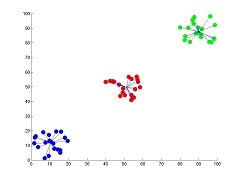
\includegraphics[width=\linewidth]{chapter1/k-means.jpg}
\end{wrapfigure}
% https://sites.google.com/site/dataclusteringalgorithms/k-means-clustering-algorithm
Кластерный анализ (англ. cluster analysis) — многомерная статистическая процедура, выполняющая сбор данных, содержащих информацию о выборке объектов, и затем упорядочивающая объекты в сравнительно однородные группы.\cite{wiki:clustering_def}

\section{Визуализация}
\subsection{Набор ирисов Фишера}

\begin{multicols}{3}
	
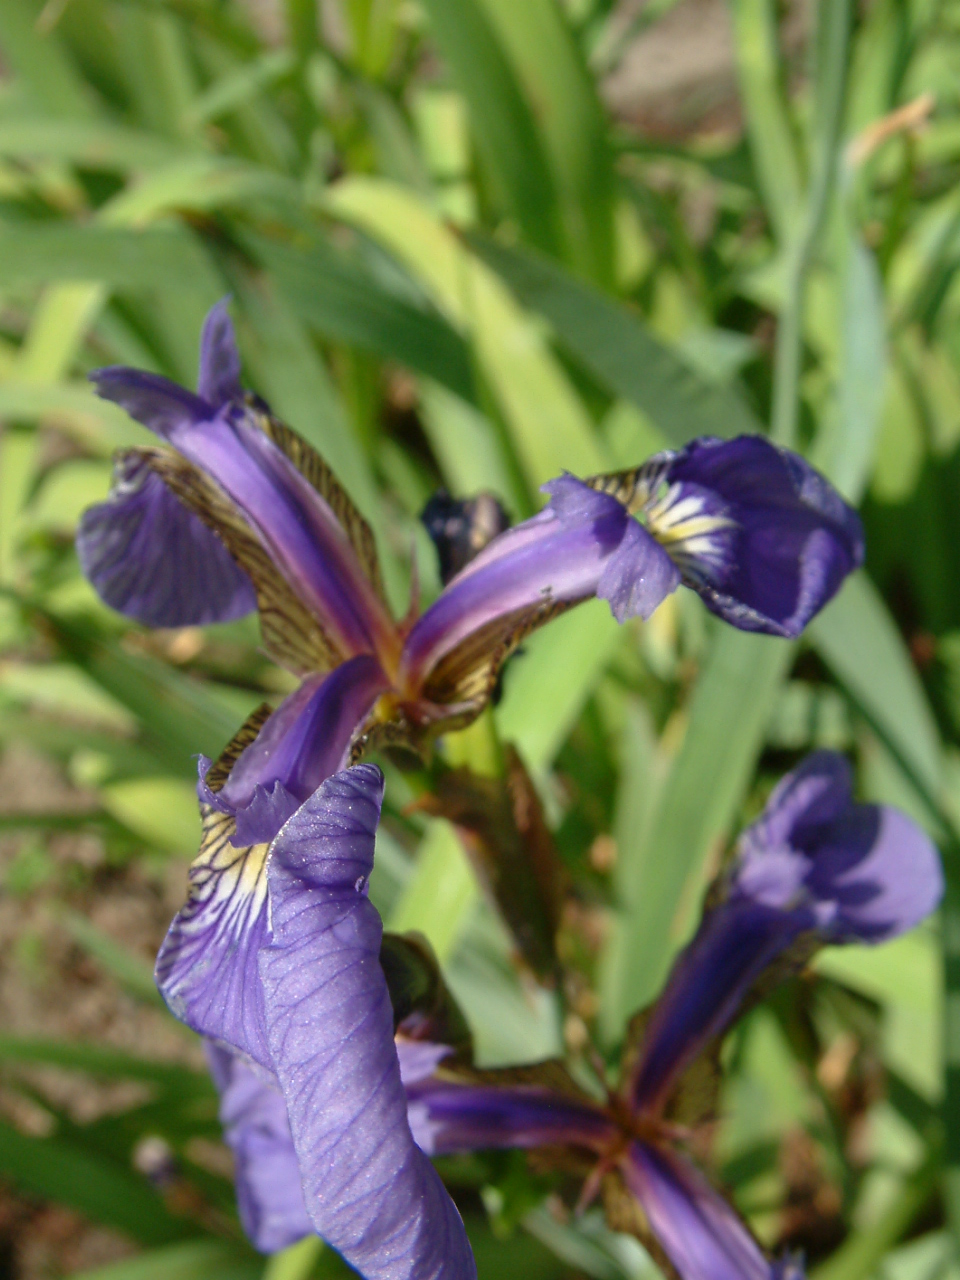
\includegraphics[height=5cm, width=4.5cm]{chapter1/Iris_setosa.jpg} %Ирис щетинистый (лат. Iris setosa)
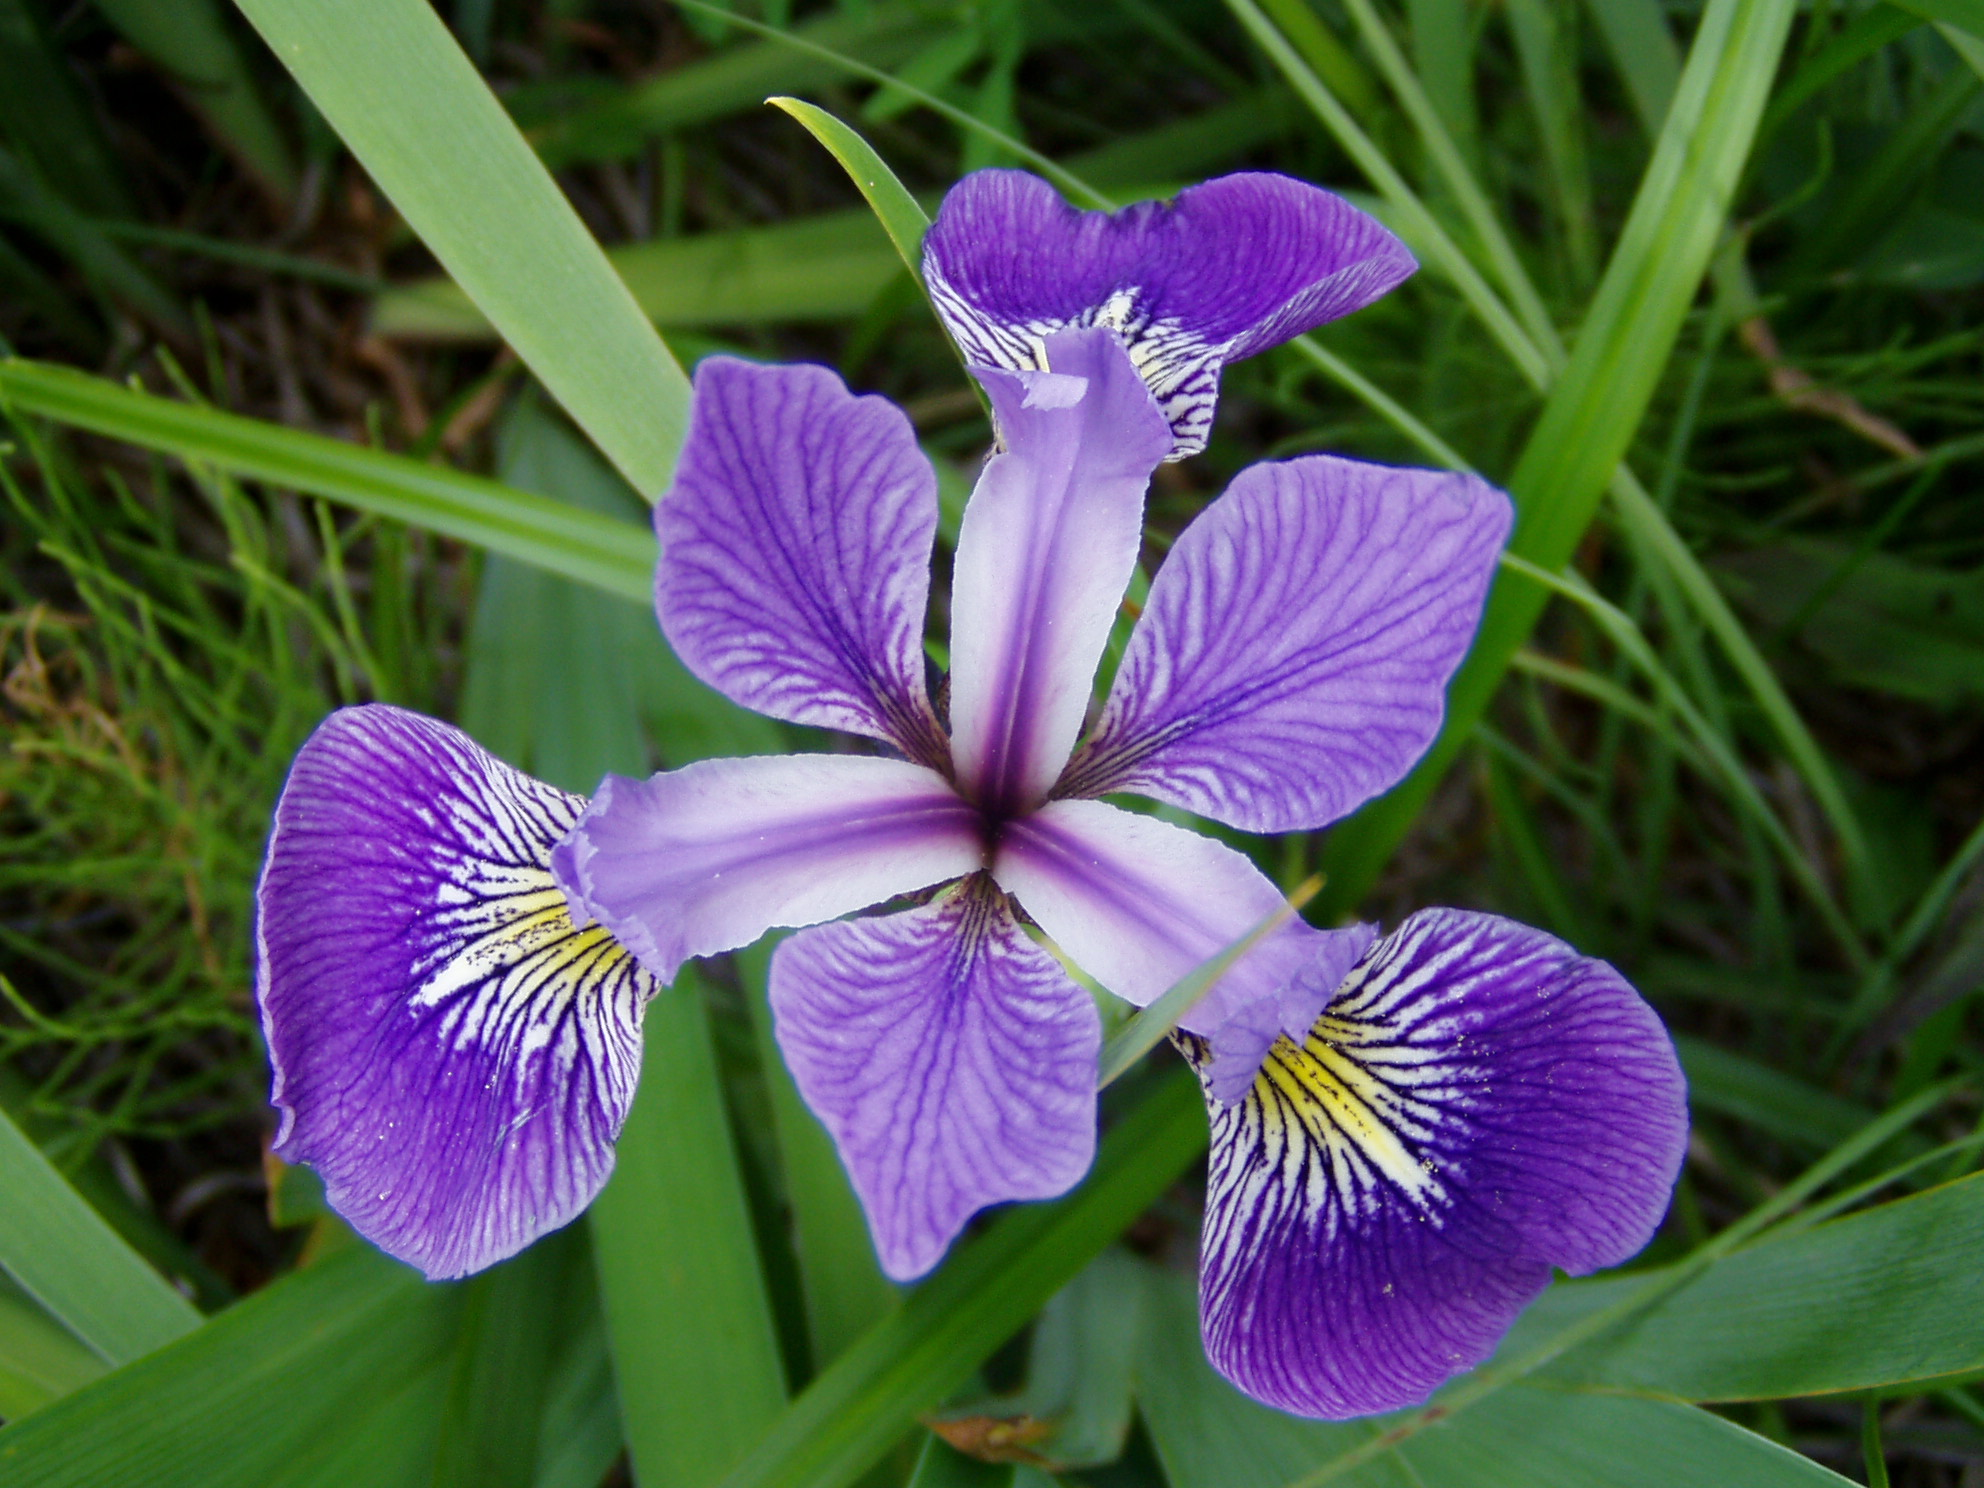
\includegraphics[height=5cm, width=4.5cm]{chapter1/Iris_versicolor.jpg} %Iris versicolor
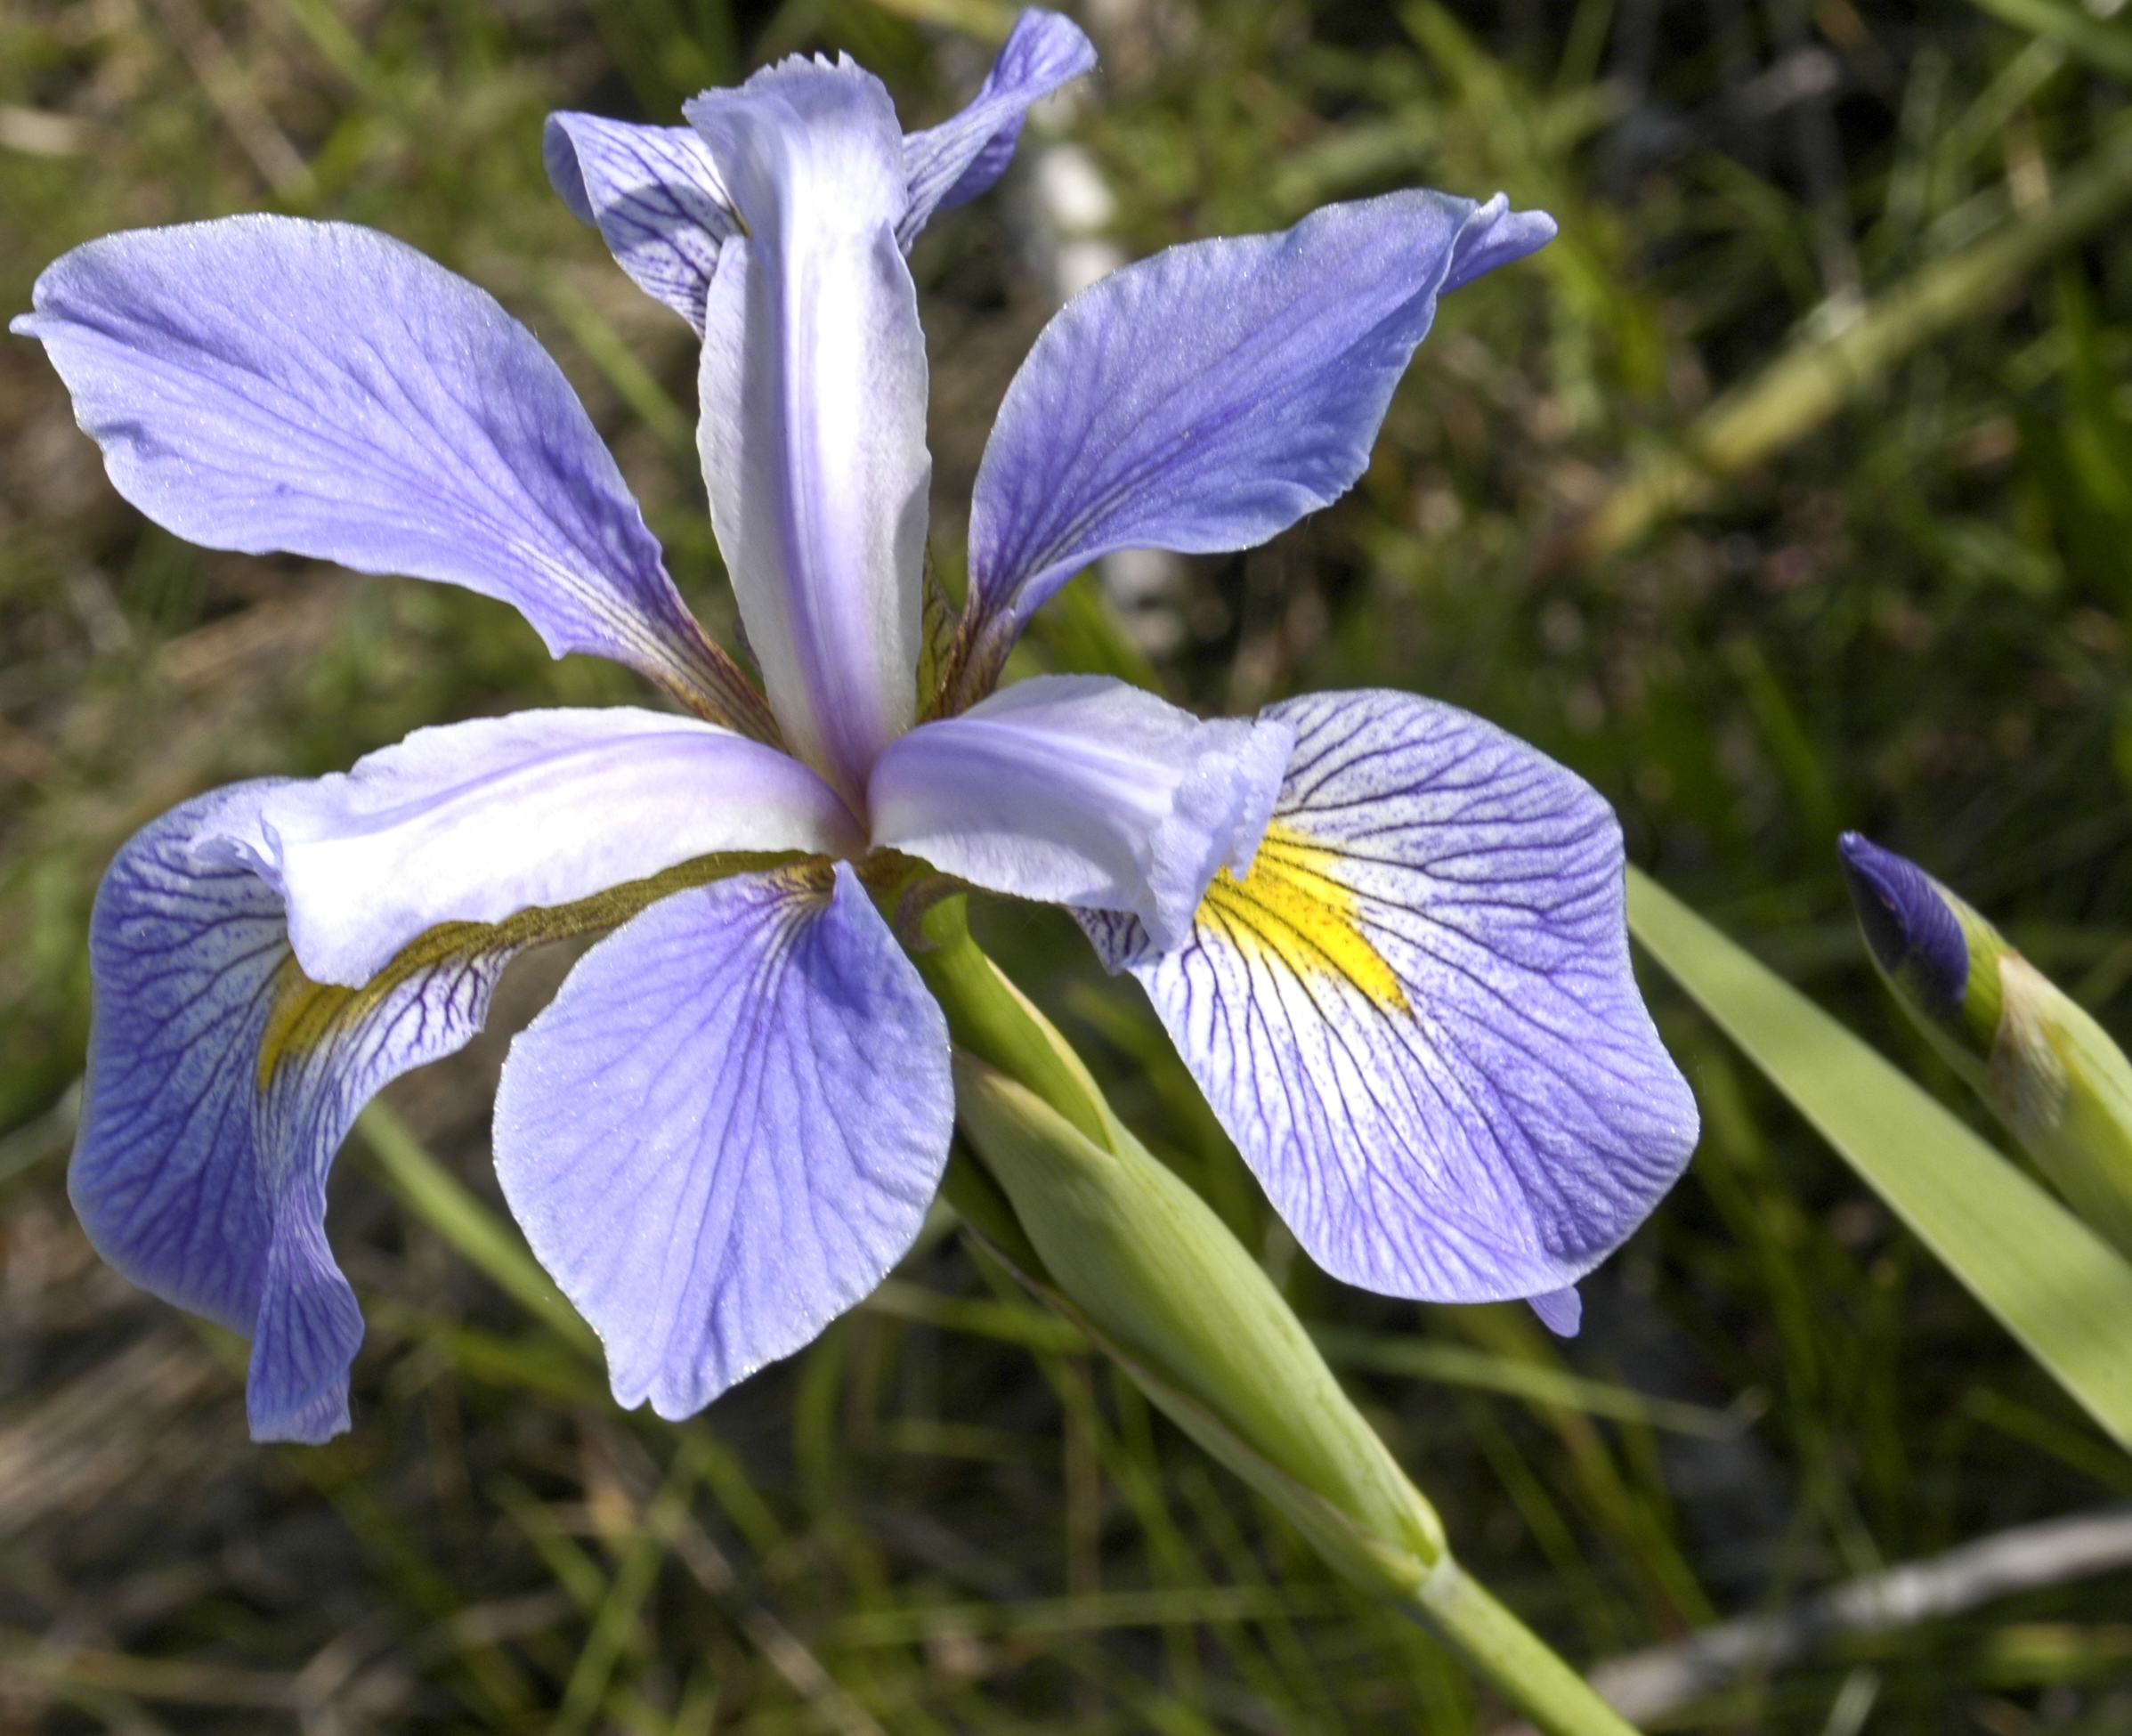
\includegraphics[height=5cm, width=4.5cm]{chapter1/Iris_virginica.jpg} %Iris virginica
\end{multicols}
    
\subsection{Примеры кода}

Задание:
\begin{itemize}
    \item Выбрать любые две пары признаков
    \item Отобразить на одном рисунке две зависимости
    \item Подписать график и оси
    \item Добавить легенду.
\end{itemize}

\section{Кластеризация}
\subsection{Методы}

Методы:
\begin{itemize}
    \item K-средних (k-means)
    \item Иерархические
\end{itemize}


\section{Машинное обучение. Определение}
Машинное обучение (англ. machine learning, ML) — класс методов искусственного интеллекта, характерной чертой которых является не прямое решение задачи, а обучение в процессе применения решений множества сходных задач. Для построения таких методов используются средства математической статистики, численных методов, методов оптимизации, теории вероятностей, теории графов, различные техники работы с данными в цифровой форме\cite{wiki:ml_def}.

Алгоритм $A$ обучается с эффективностью $E$ над данными $D$, если про росте мощности $|D|$, $E$ проявляет тенденцию к увеличению.
